\documentclass[pdf, aspectratio=169]{beamer}
\usepackage[]{hyperref,graphicx,siunitx,lmodern,booktabs,tikz,tensor}
\usepackage{pgfplots, pgfplotstable}
\usepackage{pdfpc-commands}
\usepackage[mode=buildnew]{standalone}
\mode<presentation>{\usetheme{Astro}}

\graphicspath{ {../Images/} }

\sisetup{per-mode=symbol}
\usetikzlibrary{calc,intersections, decorations.pathmorphing,shadings}
\tikzstyle{image}=[inner sep=0pt, outer sep=0pt, anchor=south west]
%\tikzstyle{proton}=[circle, minimum size = 7mm, ball color=red, black,transform shape]
%\tikzstyle{neutron}=[circle, minimum size=7mm, ball color=gray, black, transform shape]
%\tikzstyle{gammaray}=[ultra thick, -latex, decorate, decoration={snake, post length=3mm}]


%preamble
\title{All Things Bright and Beautiful}
\date{November 2, 2018}
\author{Jed Rembold}

\begin{document}
\renewcommand*{\theenumi}{\Alph{enumi}}

\begin{frame}{Announcements}
  \begin{itemize}
	  \item WebWork due on Monday
	  \item For the next few chapters we may be bouncing around a little, I'll try to keep you appraised of the relevant chapter sections
	  \item Physics Tea at 3!
	  \item Physics Seminar on laser fusion at 3:30pm in Collins 318
	\item Polling: \url{rembold-class.ddns.net}
  \end{itemize}
\end{frame}

\begin{frame}{Test Summary!}
  \begin{columns}
	\column{.7\textwidth}
	  \begin{figure}[h!]
		\centering
		\begin{tikzpicture}
		  \begin{axis}[
			width=10cm,
			height=7cm,
			xlabel= Percentile,
			ylabel= Number of Students,
			yticklabels={,,},
			ylabel near ticks,
		  ]
		  \addplot [hist={bins=7}, fill=DOrange ] table[y index=0] {../Data/Test2Data2018.csv};
		  \end{axis}
		\end{tikzpicture}
	  \end{figure}
	  \column{.3\textwidth}
	  \begin{itemize}
		\item High: 108\%
		\item Mean: 83\%
		\item Median: 86\%
	  \end{itemize}
	\end{columns}
\end{frame}

\begin{frame}{Going over test}
	Quickly going over the test to make sure everyone understands their score.
\end{frame}


\begin{frame}{Review Question}
  Which of the following is \alert{not} an always true statement about star groupings on a HR diagram (as we've drawn them)?
  \begin{enumerate}
	\item Luminous objects are toward the top
	\item Cooler objects are toward the right
	\item \alert<2>{Bluer objects are towards the bottom}
	\item Large objects are toward the upper right
  \end{enumerate}
\end{frame}

\begin{frame}{Hertzsprung-Russel Diagrams}
  \begin{center}
	\begin{tikzpicture}
	  \pgfplotsset{colormap={stars}{[0.1cm] color(0cm)=(blue); color(1.8cm)=(white); color(2.1cm)=(yellow); color(2.6cm)=(red); color(3cm)=(red!50!black)}}
	  \begin{loglogaxis}[
		  width=\textwidth,
		  height=7.5cm,
		  x dir = reverse,
		  xlabel = Temperature (K),
		  ylabel = Fraction of Sun's Luminosity,
		  ticklabel style={font=\tiny},
		  xtick = {3000, 6000, 10000, 25000},
		  xticklabels = {3000,6000,10000,25000},
		  colormap name= stars,
		  xmin = 2000,
		  xmax = 40000,
		]
		\addplot[scatter, scatter src=-x, draw=black, only marks, mark size = 1pt] table[x index=0, y index=1] {../Data/HR_Data.csv};
		\node at (axis cs: 10^4.5,10^-4) {O};
		\node at (axis cs: 10^4.2,10^-4) {B};
		\node at (axis cs: 10^3.95,10^-4) {A};
		\node at (axis cs: 10^3.85,10^-4) {F};
		\node at (axis cs: 10^3.7,10^-4) {G};
		\node at (axis cs: 10^3.6,10^-4) {K};
		\node at (axis cs: 10^3.4,10^-4) {M};
	  \end{loglogaxis}
	\end{tikzpicture}
  \end{center}
\end{frame}

%\begin{frame}{Mass and HR Diagrams}
  %\begin{itemize}
	%\item Globally, there is not an obvious trend
	%\item Trends are clear though for subgroups:
	  %\begin{itemize}
		%\item Main sequences stars decrease in mass from upper left to lower right
		%\item White dwarfs are all generally low mass
		%\item Giants and Supergiants can be any mass
	  %\end{itemize}
	%\item Mass determines where the balance point between energy in and energy out lies
	  %\begin{itemize}
		%\item More mass implies hotter and denser fusion and thus more energy
		%\item Also influences how large the star is
		%\item Lots of interacting systems striving for balance
	  %\end{itemize}
  %\end{itemize}
%\end{frame}

%\begin{frame}{Not much for Vacations}
  %\begin{columns}
	%\column{.5\textwidth}
	%\begin{itemize}
	  %\item Stars tend to live most their lives in one place on the main sequence
	  %\item Stars do not (significantly) change mass over their lifetimes
	%\end{itemize}
	%\column{.5\textwidth}
	%\begin{center}
	  %\begin{tikzpicture}
		%\clip[rounded corners] (1mm,3mm) rectangle +(68mm,68mm);
		%\node[inner sep=0pt, outer sep=0pt, anchor=south west] at (0,0) {\includegraphics[width=7cm]{ch12_lifetimes.jpg}};
	  %\end{tikzpicture}
	%\end{center}
  %\end{columns}
%\end{frame}

\begin{frame}{Shine Bright \scriptsize(like a diamond)}
  \begin{columns}
	\column{.5\textwidth}
	\begin{center}
	  \begin{tikzpicture}
		\clip[rounded corners] (1mm,3mm) rectangle +(68mm,68mm);
		\node[inner sep=0pt, outer sep=0pt, anchor=south west] at (0,0) {\includegraphics[width=7cm]{ch12_lifetimes.jpg}};
	  \end{tikzpicture}
	\end{center}
	\column{.5\textwidth}
	\begin{itemize}
	  \item A star's mass and luminosity do not increase at the same rate:
		\begin{itemize}
		  \item O star
			\begin{itemize}
			  \item $60 M_\odot$
			  \item $100000 L_\odot$
			\end{itemize}
		  \item G star
			\begin{itemize}
			  \item $1 M_\odot$
			  \item $1 L_\odot$
			\end{itemize}
		  \item M star
			\begin{itemize}
			  \item $0.2 M_\odot$
			  \item $0.01 L_\odot$
			\end{itemize}
		\end{itemize}
	  \item Brighter stars have shorter lifetimes than dimmer stars!
	\end{itemize}
  \end{columns}
\end{frame}

\begin{frame}{The End of the Line}
  \begin{itemize}
	\item What about those stars not on the main sequence?
	\item Fusing hydrogen into helium does not account for them
	\item $\Rightarrow$Stars that have exhausted their supply of hydrogen
	\item Two main types:
	  \begin{itemize}
		\item Giants
		  \begin{itemize}
			\item In crisis mode: ``Fuse all the things!''
		  \end{itemize}
		\item Dwarfs
		  \begin{itemize}
			\item In dejection, having lost all their fuel
			\item Memories of once being a Giant
		  \end{itemize}
	  \end{itemize}
  \end{itemize}
\end{frame}

\begin{frame}{Star Clusters}
  \begin{center}
	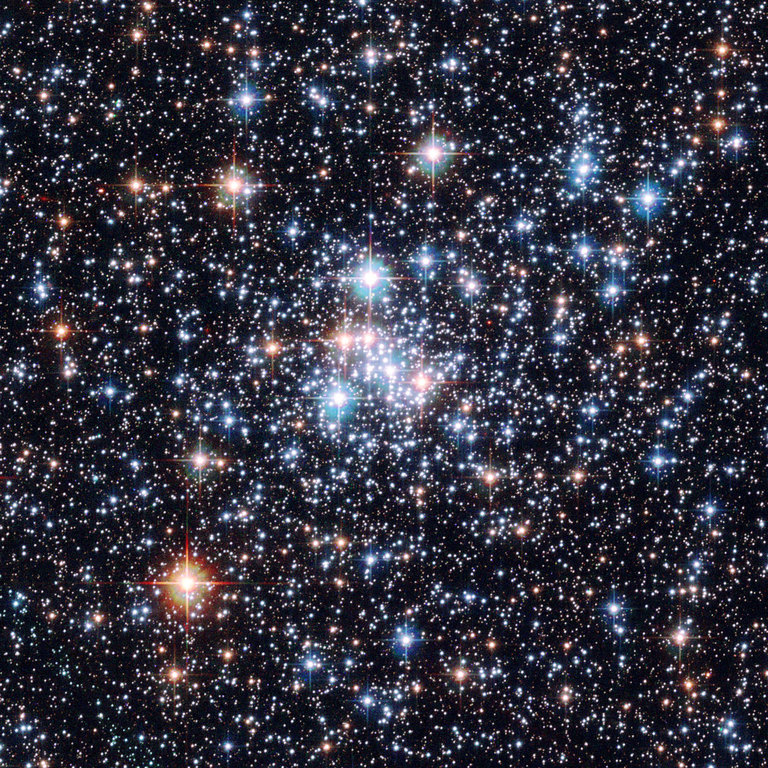
\includegraphics[width=.5\textwidth]{ch12_starcluster.jpeg}
  \end{center}
\end{frame}

\begin{frame}{Star Cluster Basics}
  \begin{itemize}
	  \item Ch 22.2
	\item All stars form from gaseous clouds
	\item So often times many can form together
	\item Why are we excited about them?
	  \begin{itemize}
		\item They are all about the same distance away.
		\item They are all about the same age.
	  \end{itemize}
	\item Main types:
	  \begin{itemize}
		\item Open clusters
		\item Globular clusters
	  \end{itemize}
  \end{itemize}
\end{frame}

\begin{frame}{Open Clusters}
  \begin{columns}
	\column{.5\textwidth}
	\begin{center}
	  \begin{tikzpicture}
		\node at (0,0) {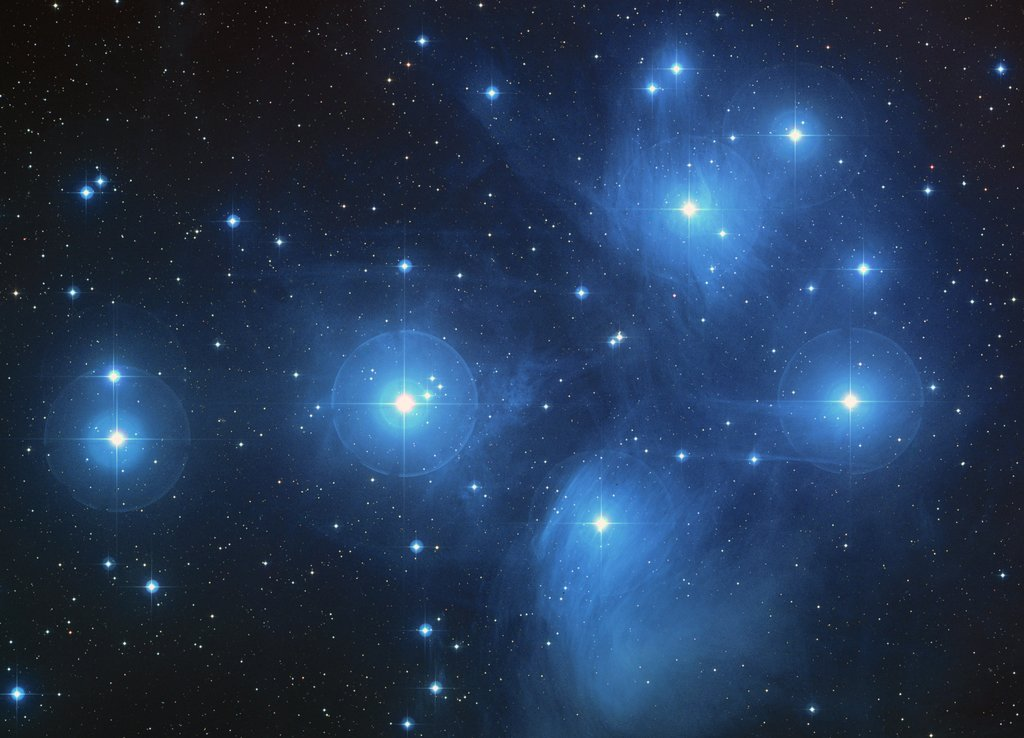
\includegraphics[width=\textwidth]{ch12_pleides.jpg}};
		\node<2> at (0,0) {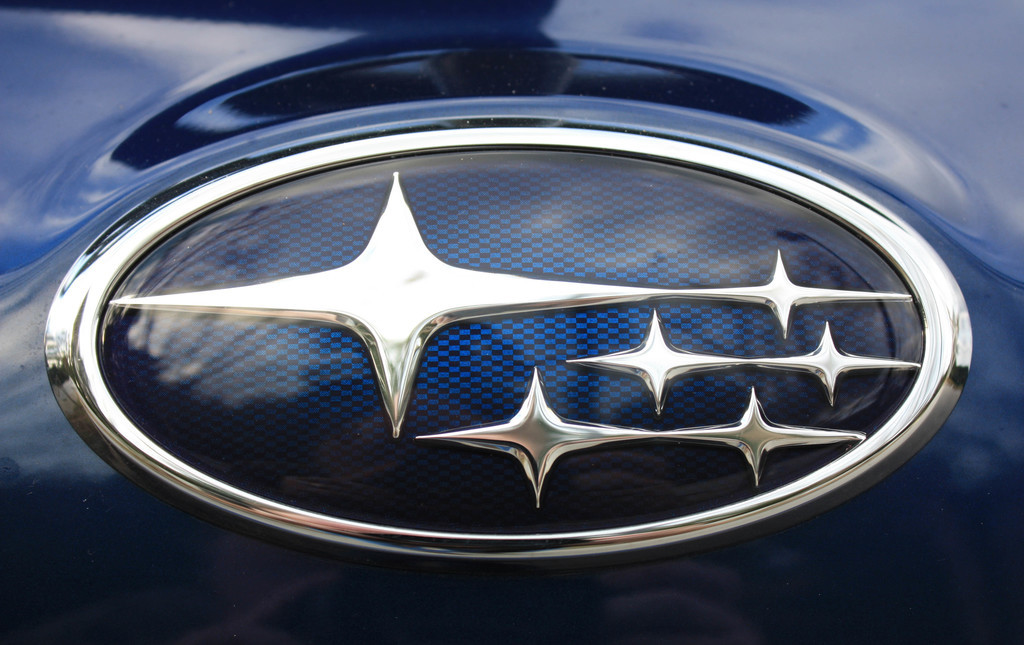
\includegraphics[width=\textwidth]{ch12_subaru.jpg}};
	  \end{tikzpicture}
	\end{center}
	\column{.5\textwidth}
	\begin{itemize}
	  \item Found in the galaxy disk
	  \item Up to several thousand stars
	  \item Stars tend to be young
	  \item Most famous the Pleiades cluster
		\begin{itemize}
		  \item Visible with your naked eye
		  \item Can find easily with a quick scan of the sky
		\end{itemize}
	\end{itemize}
  \end{columns}
\end{frame}

\begin{frame}{Globular Clusters}
  \begin{columns}
	\column{.5\textwidth}
	\begin{itemize}
	  \item Generally found in the galaxy halo
		\begin{itemize}
		  \item Above or below the disk
		\end{itemize}
	  \item Much older stars
	  \item A very concentrated density of stars
	  \item My favorite is M13, in the constellation Hercules
	\end{itemize}
	\column{.5\textwidth}
	\begin{center}
	  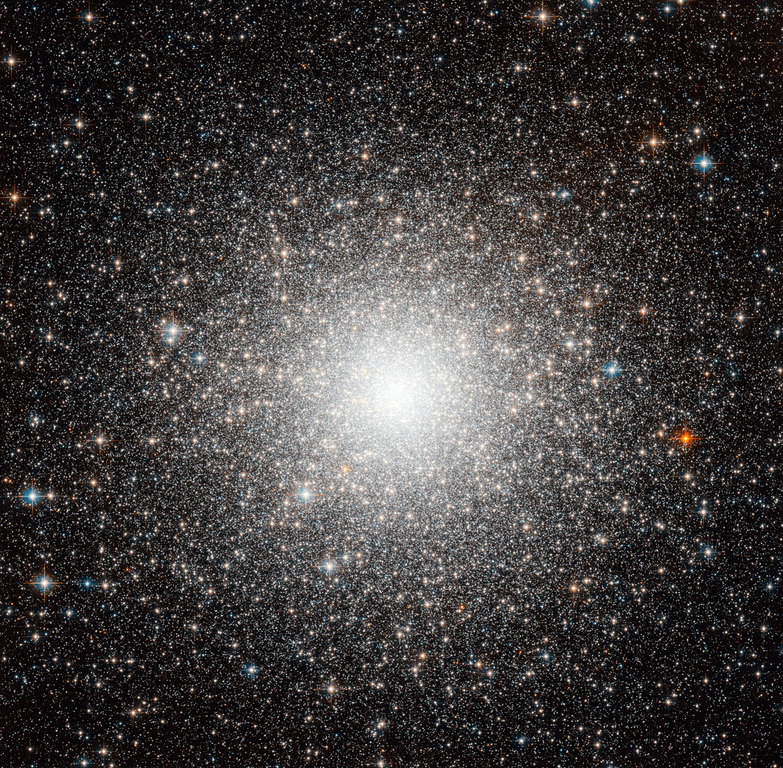
\includegraphics[width=\textwidth]{ch12_globular_cluster.jpg}
	\end{center}
  \end{columns}
\end{frame}

\begin{frame}{Getting Carded}
  \begin{itemize}
	\item Clusters are all generally about the same age
	\item A small amount of variation
	\item Should mostly be in the ``same phase of life''
	\item But brighter stars should show their age quicker!
	\item The key question:
	  \begin{itemize}
		\item Where do the cluster stars leave the Main Sequence?
	  \end{itemize}
  \end{itemize}
\end{frame}

\begin{frame}{The Pleiades}
  \begin{center}
	\begin{tikzpicture}
	  \pgfplotsset{colormap={stars}{[0.1cm] color(0cm)=(blue!50!white); color(1cm)=(white); color(2.1cm)=(yellow); color(2.6cm)=(red); color(3cm)=(red!50!black)}}
	  \begin{loglogaxis}[
		  width=\textwidth,
		  height=7.5cm,
		  x dir = reverse,
		  xlabel = Temperature (K),
		  ylabel = Fraction of Sun's Luminosity,
		  ticklabel style={font=\tiny},
		  xtick = {3000, 6000, 10000, 25000},
		  xticklabels = {3000,6000,10000,25000},
		  colormap name= stars,
		  xmin = 2000,
		  xmax = 40000,
		  ymin = 2e-5,
		  ymax = 2e6,
		]
		\addplot[scatter, scatter src=-x, draw=black, only marks, mark size = 1pt] table[x index=0, y index=1] {../Data/Pleiades_Data.csv};
		\node at (axis cs: 10^4.5,10^-4) {O};
		\node at (axis cs: 10^4.2,10^-4) {B};
		\node at (axis cs: 10^3.95,10^-4) {A};
		\node at (axis cs: 10^3.85,10^-4) {F};
		\node at (axis cs: 10^3.7,10^-4) {G};
		\node at (axis cs: 10^3.6,10^-4) {K};
		\node at (axis cs: 10^3.4,10^-4) {M};

		\draw[orange, dashed, shorten >=-5cm] (axis cs: 40000,1e2) -- node[midway, sloped, above] {\scriptsize$10^7$ yrs} +(45:2cm);
		\draw[orange, dashed, shorten >=-5cm] (axis cs: 40000,5e-3) -- node[midway, sloped, above] {\scriptsize$10^8$ yrs} +(45:2cm);
		\draw[orange, dashed, shorten >=-6cm] (axis cs: 25000,2e-5) -- node[midway, sloped, above] {\scriptsize$10^9$ yrs} +(45:3cm);
		\draw[orange, dashed, shorten >=-5cm] (axis cs: 12000,2e-5) -- node[midway, sloped, above] {\scriptsize$10^{10}$ yrs} +(45:3cm);
		\draw[orange, dashed, shorten >=-5cm] (axis cs: 7000,2e-5) -- node[midway, sloped, above] {\scriptsize$10^{11}$ yrs} +(45:3cm);

		\draw<2>[cyan, latex-] (axis cs: 10600,5e1) --+(-1cm,-1cm) node[below,align=center, rounded corners, draw, fill=Background] {Main Sequence\\Turnoff};
	  \end{loglogaxis}
	\end{tikzpicture}
  \end{center}
\end{frame}

\begin{frame}{Globular Cluster: M55}
  \begin{center}
	\begin{tikzpicture}
	  \pgfplotsset{colormap={stars}{[0.1cm] color(0cm)=(blue!50!white); color(1cm)=(white); color(2.1cm)=(yellow); color(2.6cm)=(red); color(3cm)=(red!50!black)}}
	  \begin{loglogaxis}[
		  width=\textwidth,
		  height=7.5cm,
		  x dir = reverse,
		  xlabel = Temperature (K),
		  ylabel = Fraction of Sun's Luminosity,
		  ticklabel style={font=\tiny},
		  xtick = {3000, 6000, 10000, 25000},
		  xticklabels = {3000,6000,10000,25000},
		  colormap name= stars,
		  xmin = 2000,
		  xmax = 40000,
		  ymin = 2e-5,
		  ymax = 2e6,
		]
		\addplot[scatter, scatter src=-x, draw=black, only marks, mark size = 0.5pt] table[x index=0, y index=1] {../Data/M55_Data.csv};
		\node at (axis cs: 10^4.5,10^-4) {O};
		\node at (axis cs: 10^4.2,10^-4) {B};
		\node at (axis cs: 10^3.95,10^-4) {A};
		\node at (axis cs: 10^3.85,10^-4) {F};
		\node at (axis cs: 10^3.7,10^-4) {G};
		\node at (axis cs: 10^3.6,10^-4) {K};
		\node at (axis cs: 10^3.4,10^-4) {M};

		\draw[orange, dashed, shorten >=-5cm] (axis cs: 40000,1e2) -- node[midway, sloped, above] {\scriptsize$10^7$ yrs} +(45:2cm);
		\draw[orange, dashed, shorten >=-5cm] (axis cs: 40000,5e-3) -- node[midway, sloped, above] {\scriptsize$10^8$ yrs} +(45:2cm);
		\draw[orange, dashed, shorten >=-6cm] (axis cs: 25000,2e-5) -- node[midway, sloped, above] {\scriptsize$10^9$ yrs} +(45:3cm);
		\draw[orange, dashed, shorten >=-5cm] (axis cs: 12000,2e-5) -- node[midway, sloped, above] {\scriptsize$10^{10}$ yrs} +(45:3cm);
		\draw[orange, dashed, shorten >=-5cm] (axis cs: 7000,2e-5) -- node[midway, sloped, above] {\scriptsize$10^{11}$ yrs} +(45:3cm);

		\draw<2>[cyan, latex-] (axis cs: 8000,9e-1) --+(-1cm,0cm) node[left,align=center, rounded corners, draw, fill=Background] {Main Sequence\\Turnoff};
	  \end{loglogaxis}
	\end{tikzpicture}
  \end{center}
\end{frame}

\begin{frame}{Understanding Check!}
  \begin{columns}
	\column{.5\textwidth}
	Which of the following statements is true, given the HR diagram to the right?
	\begin{enumerate}
	  \item \alert<2>{The cyan cluster is older than the orange cluster}
	  \item No stars on the cyan cluster are on the main sequence any longer
	  \item The cyan cluster and orange cluster are the same age
	  \item The cyan cluster is definitely a open cluster
	\end{enumerate}
	\column{.5\textwidth}
	\begin{center}
	  \begin{tikzpicture}[scale=.7]
		\begin{loglogaxis}[
			x dir = reverse,
			xlabel = Temperature (K),
			ylabel = Fraction of $L_\odot$,
			xtick = {3000,6000,10000,25000},
			xticklabels = {3000,6000,10000,25000},
		  ]
		  \addplot[cyan, only marks, mark size=1pt] table[x index=0, y index=1] {../Data/Ex1_Data.csv};
		  \addplot[orange, only marks, mark size=1pt] table[x index=0, y index=1] {../Data/Ex2_Data.csv};
		\end{loglogaxis}
	  \end{tikzpicture}
	\end{center}
  \end{columns}
\end{frame}

\begin{frame}{Some additional points}
  \begin{itemize}
	\item For \alert{really} old systems, not only do we see fewer stars on the main sequence, but we start seeing stars in the dwarf star population/region
	  \begin{itemize}
		\item Implies dwarfs are likely the final resting state of at least some stars
	  \end{itemize}
	\item To summarize what we know thus far:
	  \begin{itemize}
		\item Stars spend most their time on the main sequence
		  \begin{itemize}
			\item Happily burning hydrogen in their cores
		  \end{itemize}
		\item When they run out of hydrogen, they turn off the main sequence
		  \begin{itemize}
			\item Up and to the right, implying a larger size
		  \end{itemize}
		\item At least some go from being giants to shrinking to dwarfs at the end of their life
		\item If there is another stage, the universe isn't old enough yet for us to have seen it!
	  \end{itemize}
  \end{itemize}
\end{frame}

\begin{frame}{Making a Star: Gather Your Ingredients}
  \begin{itemize}
	  \item Ch 21.1 and 21.2
	\item Stars are formed in giant molecular clouds
	  \begin{itemize}
		\item Dense, cold, dusty regions of interstellar space
	  \end{itemize}
  \end{itemize}
  \begin{center}
	\includegraphics[width=.5\textwidth]{ch12_dark_cloud.jpg}
  \end{center}
\end{frame}

\begin{frame}{Easiest to See in Infrared}
  \begin{center}
	\begin{tikzpicture}
	  \node[image] at (0,0) {\includegraphics[width=7cm]{ch12_Cloud1.png}};
	  \node<2>[image, opacity=0.5] at (0,0) {\includegraphics[width=7cm]{ch12_Cloud2.png}};
	  \node<3>[image, opacity=1.0] at (0,0) {\includegraphics[width=7cm]{ch12_Cloud2.png}};
	\end{tikzpicture}
  \end{center}
\end{frame}

\begin{frame}{Bring it in\ldots}
  \begin{itemize}
	\item Need gravity to be greater than any internal gas pressure
	  \begin{itemize}
		\item Easiest with dense, cold regions
		\item Hence the molecular clouds
	  \end{itemize}
	\item Densest regions attract the most gas
	  \begin{itemize}
		\item Breaks a cloud up into various smaller clouds
		\item Each smaller, dense cloud can continue to contract to become a protostar
	  \end{itemize}
  \end{itemize}
  \begin{center}
	\includegraphics[width=7.5cm]{ch12_orion_infrared.jpg}
  \end{center}
\end{frame}


\end{document}
